\newpage
%%%%%%%%%%%%%%%%%%%%%%%%%%%%%%%%%%%%%%%%%%%%%%%%%%%%%%%%%%%%%%%%%%%%%%%%%%%
\section{Textausgabe mit Bitmaps}
%\subsection{Ein Beispiel}
Oft erfolgen Textausgaben nicht über Fonts, sondern über eine \gls{spritelib}. In einer solchen befinden sich dann Schriftzeichen, Symbole oder Ziffern, die dann meist auch in einem besonderen dem Spiel angepassten Design sind. In \abbref[vref]{picSpritelib01} finden Sie eine Spritelib, die Sprites für ein Kampfspiel des 2.~Weltkriegs zur Verfügung stellt. Unter anderem sind dort die Sprites für die Ziffern $0-9$ und die Buchstaben des lateinischen Alphabets zu finden. Ein Vorteil dieses Vorgehens ist, dass das Vorhandensein des Spielfonts nicht vorausgesetzt werden muss. Wenn Sie also die Textausgabe mit dem Font \emph{Calibri} durchführen, muss dieser Font ja auf dem Zielrechner installiert sein. Nachteil ist, dass sich Bitmaps meist nur sehr schlecht skalieren lassen und dann kaum Schriften verschiedener Größen zur Verfügung stehen. 

Die Idee ist nun, die einzelnen Buchstaben aus der Spritelib auszustanzen und in einer geschickten Datenstruktur abzulegen. Soll nun ein Text ausgegeben werden, wird der Text in seine Buchstaben zerlegt und die dazu passenden Buchstabensprites aus der Datenstruktur auf ein Zielbitmap -- beispielsweise Screen -- ausgegeben. Ich möchte das ganze hier an einem einfachen Beispiel aufzeigen. Basis ist eine Spritelib mit einem Zeichensatz in fünf verschiedenen Farben (siehe \abbref[vref]{picTextbitmaps01}).

\myebild{1945}{0.53}{Beispiel für eine Spritelib}{picSpritelib01}

Der erste Teil von \srcref[vref]{srcTextbitmaps00a} sollte bekannt vorkommen und ist nur um einige Bequemlichkeiten erweitert worden. Die Pfadangaben lasse ich mir nun in den statischen Methoden \texttt{filepath()} und \texttt{imagepath()} ermitteln.

\lstsource{SRC/00 Einführung/08 TextBitmaps/textbitmaps.py}{1}{21}{python}{Textbitmaps (1), Präambel und \texttt{Settings}}{srcTextbitmaps00a} 

Die Klasse \texttt{Spritelib} wird eigentlich nur als Container gebraucht. Sie lädt sich die Spritelib der Buchstaben und Symbole und enthält einige Angaben, die ich brauche, um ganz gezielt einzelne Buchstaben oder Symbole auszustanzen:

\begin{itemize}
    \item \texttt{nof}: Enthält die Anzahl der Zeilen und Spalten. Unser Symbolsatz ist im Bitmap in 4~Zeilen und 10~Spalten angeordnet. Da ich mich immer nur für eine Farbe interessiere, reicht mir das.

    \item \texttt{letter}: Jedes Sprite hat eine Breite und eine Höhe. In unserem Fall kommt erleichternd hinzu, dass alle Sprites immer den gleichen Platzbedarf haben; schauen Sie sich dazu die drei Quadrate um die Buchstaben~\texttt{N},~\texttt{W} und~\texttt{X} in \abbref[vref]{picSpritelib02} an. Unsere Sprites haben alle eine Breite und eine Höhe von $18~px$.

    \item \texttt{offset}: Das erste Sprite oben links hat einen Abstand vom linken Rand und einen vom oberen Rand. Schauen Sie sich dazu das Sprite der Zahl~\texttt{0} in \abbref{picSpritelib02} an. Dort haben wir das Quadrat um das Bitmap und zwischen dem Quadrat und der oberen bzw. der linken Kante einen Abstand (markiert durch die grüne Linie). Beide Offsets haben in unserem Beispiel einen Wert von $6~px$.

    \item \texttt{distance}: Jedes Sprite hat einen Abstand zum nächsten Sprite nach rechts und nach unten. Zum Glück sind unsere Sprites äquidistant in der Spritelib abgelegt, so dass ich es hier recht einfach habe. Am Beispiel des Sprites für~\texttt{X} in \abbref{picSpritelib02} können Sie die Abstände sehen. Hier sind es jeweils $14~px$.
\end{itemize}


\begin{figure}[H]
\begin{center}
\begin{tikzpicture}
\node (myfirstpic) at (1cm,-1cm) {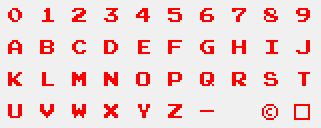
\includegraphics[scale=1.2]{symbole_rot.png}};

\draw
 (-4.2cm, 1.5cm) node (a) {}
 ( 6.15cm,1.5cm) node (b) {}
 (-4.2cm, 1.2cm) node (c) {}
 (-4.2cm,-3.2cm) node (d) {}
;
\draw 
 (-0.73, -2.65) node (X) {}
 (-0.72, -2.44)[inner sep=0, outer sep=0] node (XL) {}
 (-0.52, -2.22)[inner sep=0, outer sep=0] node (XT) {}

 (-0.73, -1.67) node (N) {}

 (-1.71, -2.65) node (W) {}

 (-3.66,  0.28) node (O) {}
 (-3.45,  0.71) node (OT) {}
 (-3.65,  0.5) node (OL) {}
;



\draw[>-<, very thick, blue, densely dotted] 
 (a) --  
 node[above, blue, xshift=0cm] {nof['cols']}
 (b)
;
\draw[>-<, very thick, blue, densely dotted] 
 (c) --  
 node[left, blue, xshift=0cm] {nof['rows']}
 (d)
;
\draw (X) rectangle +(0.44cm, 0.44cm);
\draw (N) rectangle +(0.44cm, 0.44cm);
\draw (W) rectangle +(0.44cm, 0.44cm);
\draw (O) rectangle +(0.44cm, 0.44cm);

\draw[very thick, green] 
 (OL) -- 
 node[below, green, yshift=-0.2cm, xshift=0.4cm] {\tiny offset['h']}
 +(-0.24cm, 0.0cm);

\draw[very thick, green]
 (OT) -- 
 node[right, green, yshift=0.0cm, xshift=0cm] {\tiny offset['v']}
 +( 0.0cm, 0.24cm);

\draw[very thick, green] 
 (XL) -- 
 node[below, green, yshift=-0.1cm] {\footnotesize distance['h']}
 +(-0.54cm, 0.0cm);

\draw[very thick, green] 
 (XT) --  
 node[right, green, xshift=0cm] {\footnotesize distance['v']} 
+( 0.0cm,  0.54cm);

\end{tikzpicture}
\caption{Bedeutung der Angaben in \texttt{Spritelib}}\label{picSpritelib02}
\end{center}
\end{figure}


\lstsource{SRC/00 Einführung/08 TextBitmaps/textbitmaps.py}{24}{36}{python}{Textbitmaps (2), \texttt{Spritelib}}{srcTextbitmaps00b} 

Kommen wir jetzt zur eigentlich interessanten Klasse: \texttt{Letters}. Diese stanzt aus der Spritelib alle Sprites einer Farbe aus und stellt sie in einem \gls{dictionary}\index{Dictionary} als \texttt{Surface}-Objekte zur Verfügung. Dabei wird eine Menge rumgerechnet, was Sie aber nicht abschrecken sollte; es ist letztlich Grundschulmathematik. Fangen wir mit dem Konstruktor an. Der Konstruktor hat zwei Übergabeparameter: Der erste Parameter \texttt{spritelib} ist ein Verweis auf das \texttt{Spritelib}-Objekt, welches das originale Bitmap geladen hat und einige Abstandsinformationen enthält. Der zweite Parameter \texttt{colornumber} ermöglicht es mir später nur für eine Farbe den vollständigen Symbolsatz auszulesen: \texttt{0} steht für die weißen Sprites, \texttt{1} für die gelben usw..

\lstsource{SRC/00 Einführung/08 TextBitmaps/textbitmaps.py}{39}{45}{python}{Textbitmaps (3): Konstruktor von \texttt{Letters}}{srcTextbitmaps00c} 

In der Methode \texttt{create\_letter\_bitmap()} werden nun die einzelnen Sprites ausgestanzt und in ein Dictionary abgelegt. Die Indizes des Dictionaries werden in \zeiref{srcTextbitmaps0000} definiert. Hier muss die Reihenfolge natürlich der entsprechen, mit der man die Sprites ausstanzt. Die Variable \texttt{index} sorgt genau dafür, dass bei jedem Schleifendurchlauf der nächste \texttt{lettername} als Schlüssel für das Dictionary verwendet wird.

In \zeiref{srcTextbitmaps0001} wird die Position, also die Pixelkoordinaten des ersten Sprites ausgerechnet. Versuchen Sie doch selbst anhand der Angaben in \abbref[vref]{picSpritelib02} die Arithmetik nachzuvollziehen! Nur Mut, sie ist nicht schwierig, sondern nur lang.

Ab \zeiref{srcTextbitmaps0002} beginnt eine verschachtelte \forSchleife. Die äußere Schleife durchläuft alle Zeilen der Spritelib und die innere die Spalten. Ziel dieser Konstruktion ist es, für jedes Sprite ein \texttt{Rect}-Objekt zu erzeugen, in welchem ich die Position und die Größe des Sprites abspeichere. In \zeiref{srcTextbitmaps0003} wird die obere Koordinate und in \zeiref{srcTextbitmaps0005} die linke Koordinate der Position berechnet. Wenn Sie \zeiref{srcTextbitmaps0001} verstanden haben, sollten diese beiden Berechnungen keine Schwierigkeiten mehr bereiten. Höhe und Breite in \zeiref{srcTextbitmaps0005} sind einfach, da alle Sprites immer die gleichen Größen haben. Anschließend wird das \texttt{Rect}-Objekt erzeugt und zum Ausstanzen des Bitmap mit Hilfe von \texttt{subsurface()}\myindex{pyg}{\texttt{Surface}!\texttt{subsurface()}} verwendet. Dieses ausgestanzte Bitmap wird dann unter seinem Symbolnamen im Dictionary abgelegt.

\lstsource{SRC/00 Einführung/08 TextBitmaps/textbitmaps.py}{47}{62}{python}{Textbitmaps (4): \texttt{create\_letter\_bitmap()} von \texttt{Letters}}{srcTextbitmaps00d} 

Die Methode \texttt{get\_text()} liefert mir letztlich die passende Bitmap-Folge zu einem Text. Dabei bedient sie sich der Methode \texttt{get\_letter()}, die notwendig ist, damit das Programm nicht bei undefinierten Buchstaben/Symbolen abstürzt. Wenn Sie jetzt beispielsweise ein \texttt{ü} eintippen, wird das Quadrat ausgegeben.

\lstsource{SRC/00 Einführung/08 TextBitmaps/textbitmaps.py}{64}{77}{python}{Textbitmaps (5): \texttt{get\_letter()} und \texttt{get\_text()} von \texttt{Letters}}{srcTextbitmaps00e} 


Das eigentliche Hauptprogramm ist in der Klasse \texttt{TextBitmaps} gekapselt. Da die Quelltexte hier nichts neues beinhalten, sollte der Quelltext verstanden werden. Nur zwei Zeilen möchte ich näher besprechen:

\begin{itemize}
    \item \zeiref{srcTextbitmaps0008}: Hier wird das \gls{slicing} von \glspl{array} verwendet. Die Angabe~\texttt{-1} bewirkt, dass der Ende-Zeiger des Slice beim letzten Element startet und dann einen Schritt nach links geht. Das Ergebnis ist ein um das letzte Zeichen gekürzter neuer String.

    \item \zeiref{srcTextbitmaps0009}: Das Attribut \texttt{unicode}\myindex{pyg}{\texttt{event}!\texttt{Event}!\texttt{unicode}}\randnotiz{unicode} liefert mir, sofern dies sinnvoll ist, den Wert der gedrückten Tastatur im \gls{unicode}-Format. Somit werden sinnvolle Buchstaben, Ziffern usw. als Zeichen meinem String hinzugefügt.
\end{itemize}

\lstsource{SRC/00 Einführung/08 TextBitmaps/textbitmaps.py}{80}{115}{python}{Textbitmaps (6): \texttt{TextBitmaps}}{srcTextbitmaps00f}

%Und der Vollständigkeit halber:

%\lstsource{SRC/00 Einführung/08 TextBitmaps/textbitmaps.py}{118}{999}{python}{Textbitmaps (7): Hauptprogramm}{srcTextbitmaps00g}

\myebild{textbitmaps00}{0.7}{Textausgabe mit Bitmaps}{picTextbitmaps01}

\subsection*{Was war neu?}

Textausgaben werden nicht nur über Fonts erzeugt, sondern auch über Spritlibs, die Zeichenbitmaps enthalten. Diese werden ausgestanzt und neuen Bitmaps zusammengesetzt.

Es wurden folgende Pygame-Elemente eingeführt:

\begin{itemize}
	\item \texttt{pygame.event.Event.unicode}:
	\myindex{pyg}{\texttt{event}!\texttt{Event}!\texttt{unicode}}\\ \url{https://www.pygame.org/docs/ref/event.html}

	\item \texttt{pygame.Surface.subsurface()}:
	\myindex{pyg}{\texttt{Surface}!\texttt{subsurface()}}\\ \url{https://www.pygame.org/docs/ref/surface.html#pygame.Surface.subsurface}
	
\end{itemize}
